\begin{frame}[label=u2_thanks]{\strut}
\centering\vfill
\makebox[\textwidth][c]{%
\begin{beamercolorbox}[wd=0.68\textwidth,sep=1.2em,center,rounded=true,shadow=true]{block body}
{\LARGE\bfseries Thanks for listening!}\par\vspace{1em}
{\large Reporter: Lekai Yao}\par\vspace{0.45em}
{\large 2026.9.24}
\end{beamercolorbox}}
\vfill
\end{frame}

\appendix
\begin{frame}[label=u2_selection_1]{Five variables, all pthat: training}
\begin{columns}[T]
\column{0.46\textwidth}\small
\textbf{Common training selection}
\begin{center}
\begin{tabular}{@{}ll@{}}\toprule
Variable & Selection before ML\\\midrule
\var{Bpt} & $15 < \var{Bpt} < 50$ GeV\\
\var{By} & $|\var{By}| < 1.6$\\
\var{BQvalue} & $\var{BQvalue} < 0.15$ GeV\\
\var{Btrk2dR} & $\var{Btrk2dR} < 0.35$\\\bottomrule
\end{tabular}\end{center}
\column{0.50\textwidth}\small
\textbf{Input variables}\par\medskip
\var{Btrk1dR}, \var{Btrk2Pt}\par
\var{BtrkPtimb}, \var{Bmu1pt}\par
\var{Bmu2pt}\par\medskip
\textbf{X MC:} All pthat components retained.\par
\var{pThatreweight}; no extra reweighting.\par
No additional signal training mass window.\par\medskip
\textbf{DATA training background}\par
$(3.80,3.85)\cup(3.89,3.94)$ GeV.\par
Unit weights; same common selection.
\end{columns}
\end{frame}

\begin{frame}[label=u2_punzi_1]{Five variables, all pthat: Punzi FOM}
\begin{columns}[T]
\column{0.68\textwidth}\centering
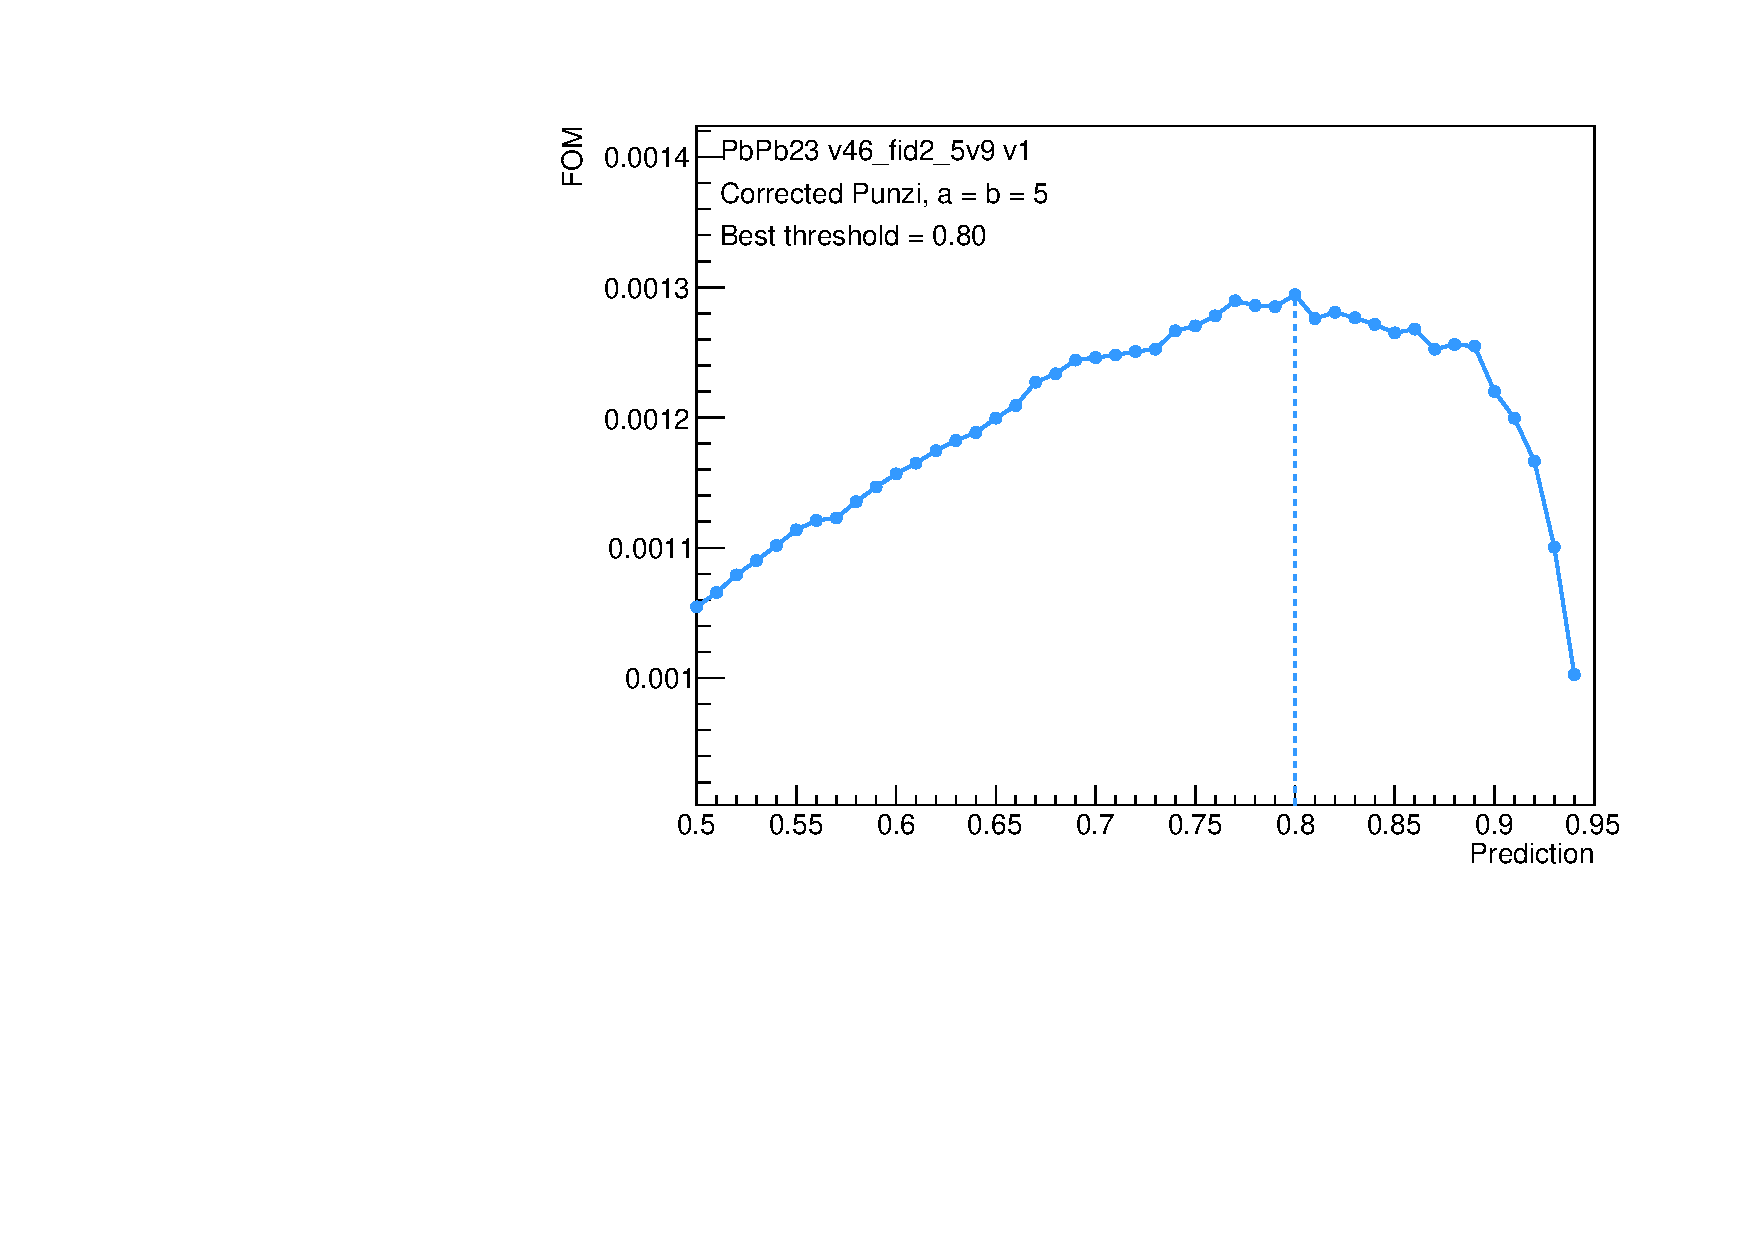
\includegraphics[width=\linewidth,height=0.73\textheight,keepaspectratio]{figures/20260924/backup_5v9_punzi_score.pdf}
\column{0.29\textwidth}\small
\textbf{Empirical corrected Punzi}\par
$a=b=5$.\par\medskip
Score: 0.50--0.95\par
Step: 0.01\par\medskip
\textbf{Grid maximum}\par
score $>0.80$\par
FOM $=1.294304\times10^{-3}$\par\medskip
\end{columns}
\end{frame}

\begin{frame}[label=u2_fit_1]{Five variables, all pthat: optimal two-peak fit}
\begin{columns}[T]
\column{0.65\textwidth}\centering
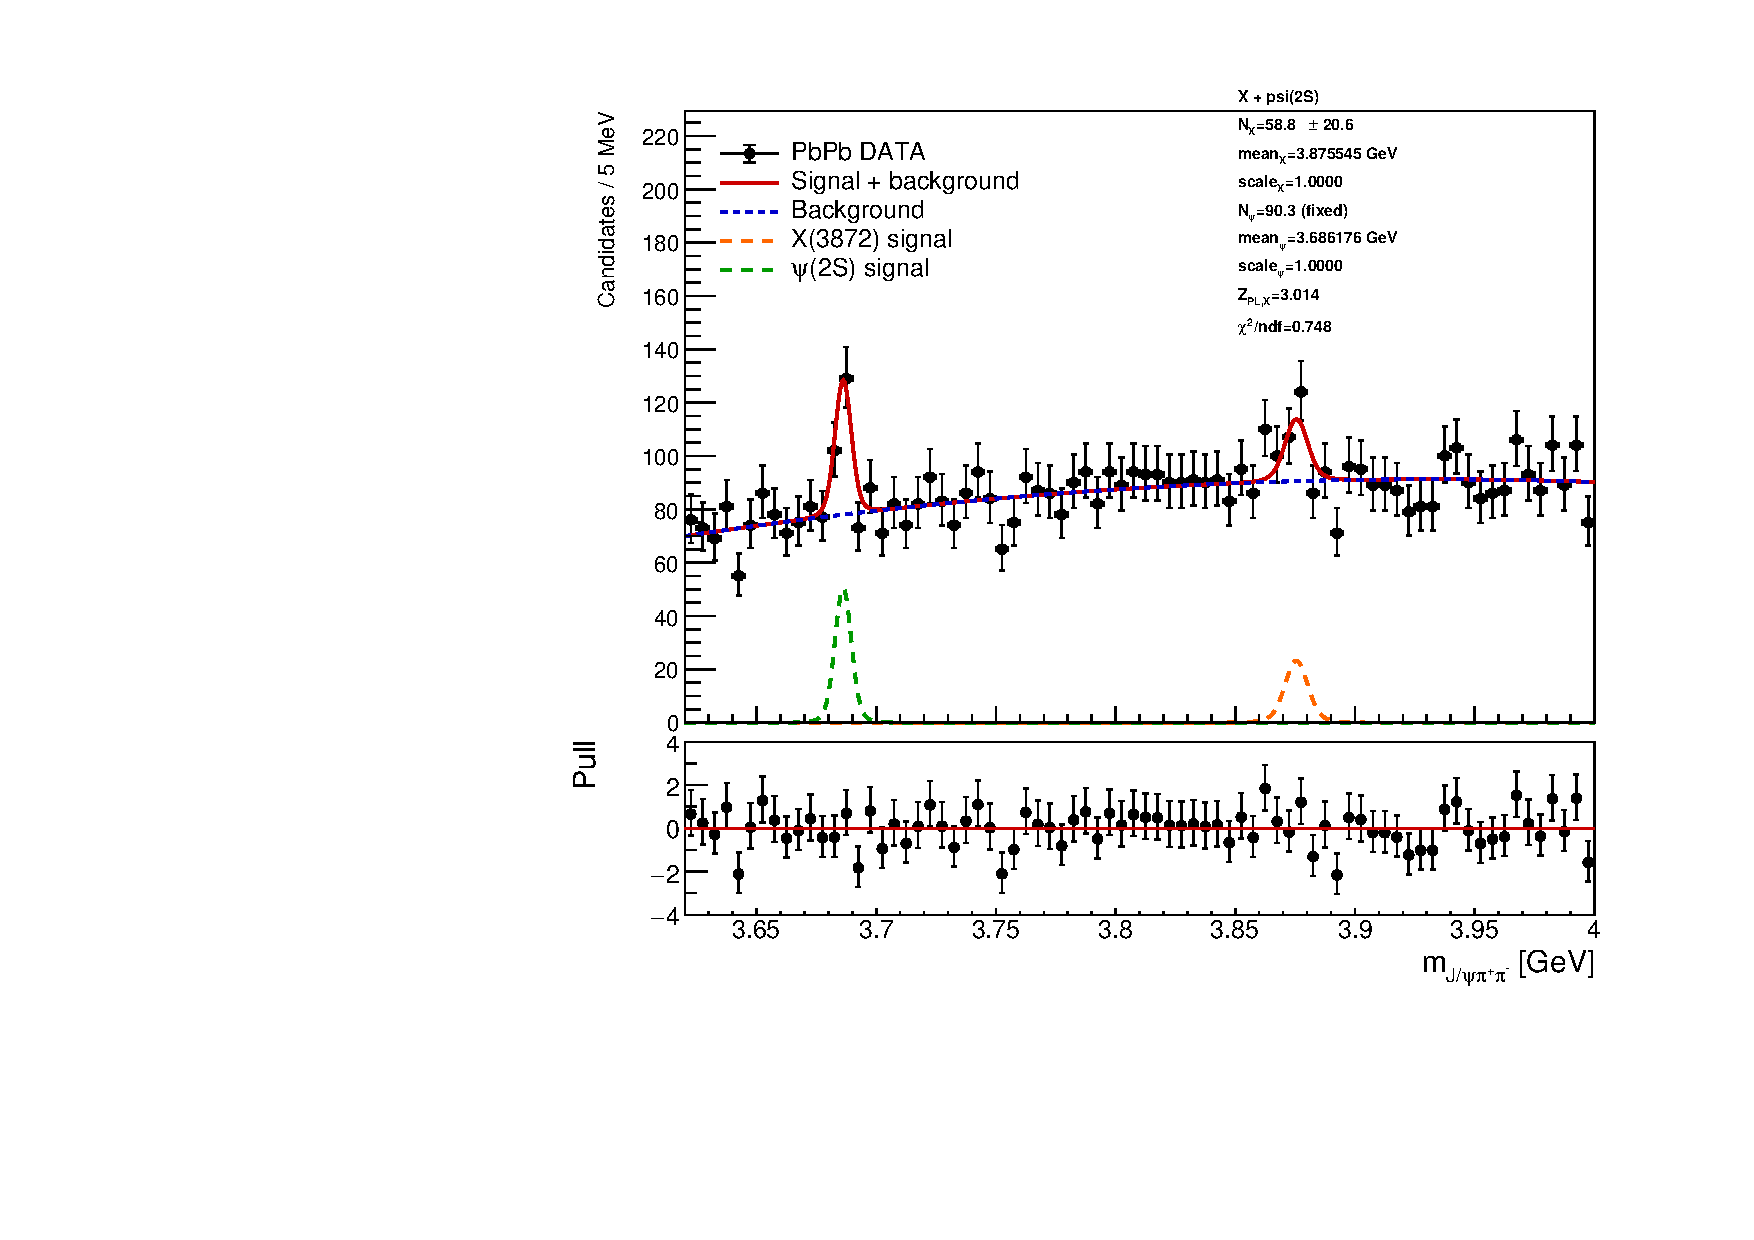
\includegraphics[width=\linewidth,height=0.72\textheight,keepaspectratio]{figures/20260924/backup_5v9_conditional_fit.pdf}
\column{0.32\textwidth}\small
\textbf{score $>0.80$}\par\medskip
$N_X=58.83\pm20.60$\par
$N_{\psi(2S)}=90.33$ (fixed)\par\medskip
$\sqrt{q_0}=3.014$\par
\medskip
MC double-Gaussian widths fixed.\par
2nd-order Chebyshev background.
\end{columns}
\end{frame}

\begin{frame}[label=u2_selection_2]{Six variables, pthat5 excluded: training}
\begin{columns}[T]
\column{0.46\textwidth}\small
\textbf{Common training selection}
\begin{center}
\begin{tabular}{@{}ll@{}}\toprule
Variable & Selection before ML\\\midrule
\var{Bpt} & $15 < \var{Bpt} < 50$ GeV\\
\var{By} & $|\var{By}| < 1.6$\\
\var{BQvalue} & $\var{BQvalue} < 0.15$ GeV\\
\var{Btrk2dR} & $\var{Btrk2dR} < 0.35$\\\bottomrule
\end{tabular}\end{center}
\column{0.50\textwidth}\small
\textbf{Input variables}\par\medskip
\var{Btrk1dR}, \var{Btrk2Pt}\par
\var{BtrkPtimb}, \var{Bcos_dtheta}\par
\var{Bmu1pt}, \var{Bmu2pt}\par\medskip
\textbf{X MC:} pthat5 excluded in training and application.\par
\var{pThatreweight}; no extra reweighting.\par
No additional signal training mass window.\par\medskip
\textbf{DATA training background}\par
$(3.80,3.85)\cup(3.89,3.94)$ GeV.\par
Unit weights; same common selection.
\end{columns}
\end{frame}

\begin{frame}[label=u2_punzi_2]{Six variables, pthat5 excluded: Punzi FOM}
\begin{columns}[T]
\column{0.68\textwidth}\centering
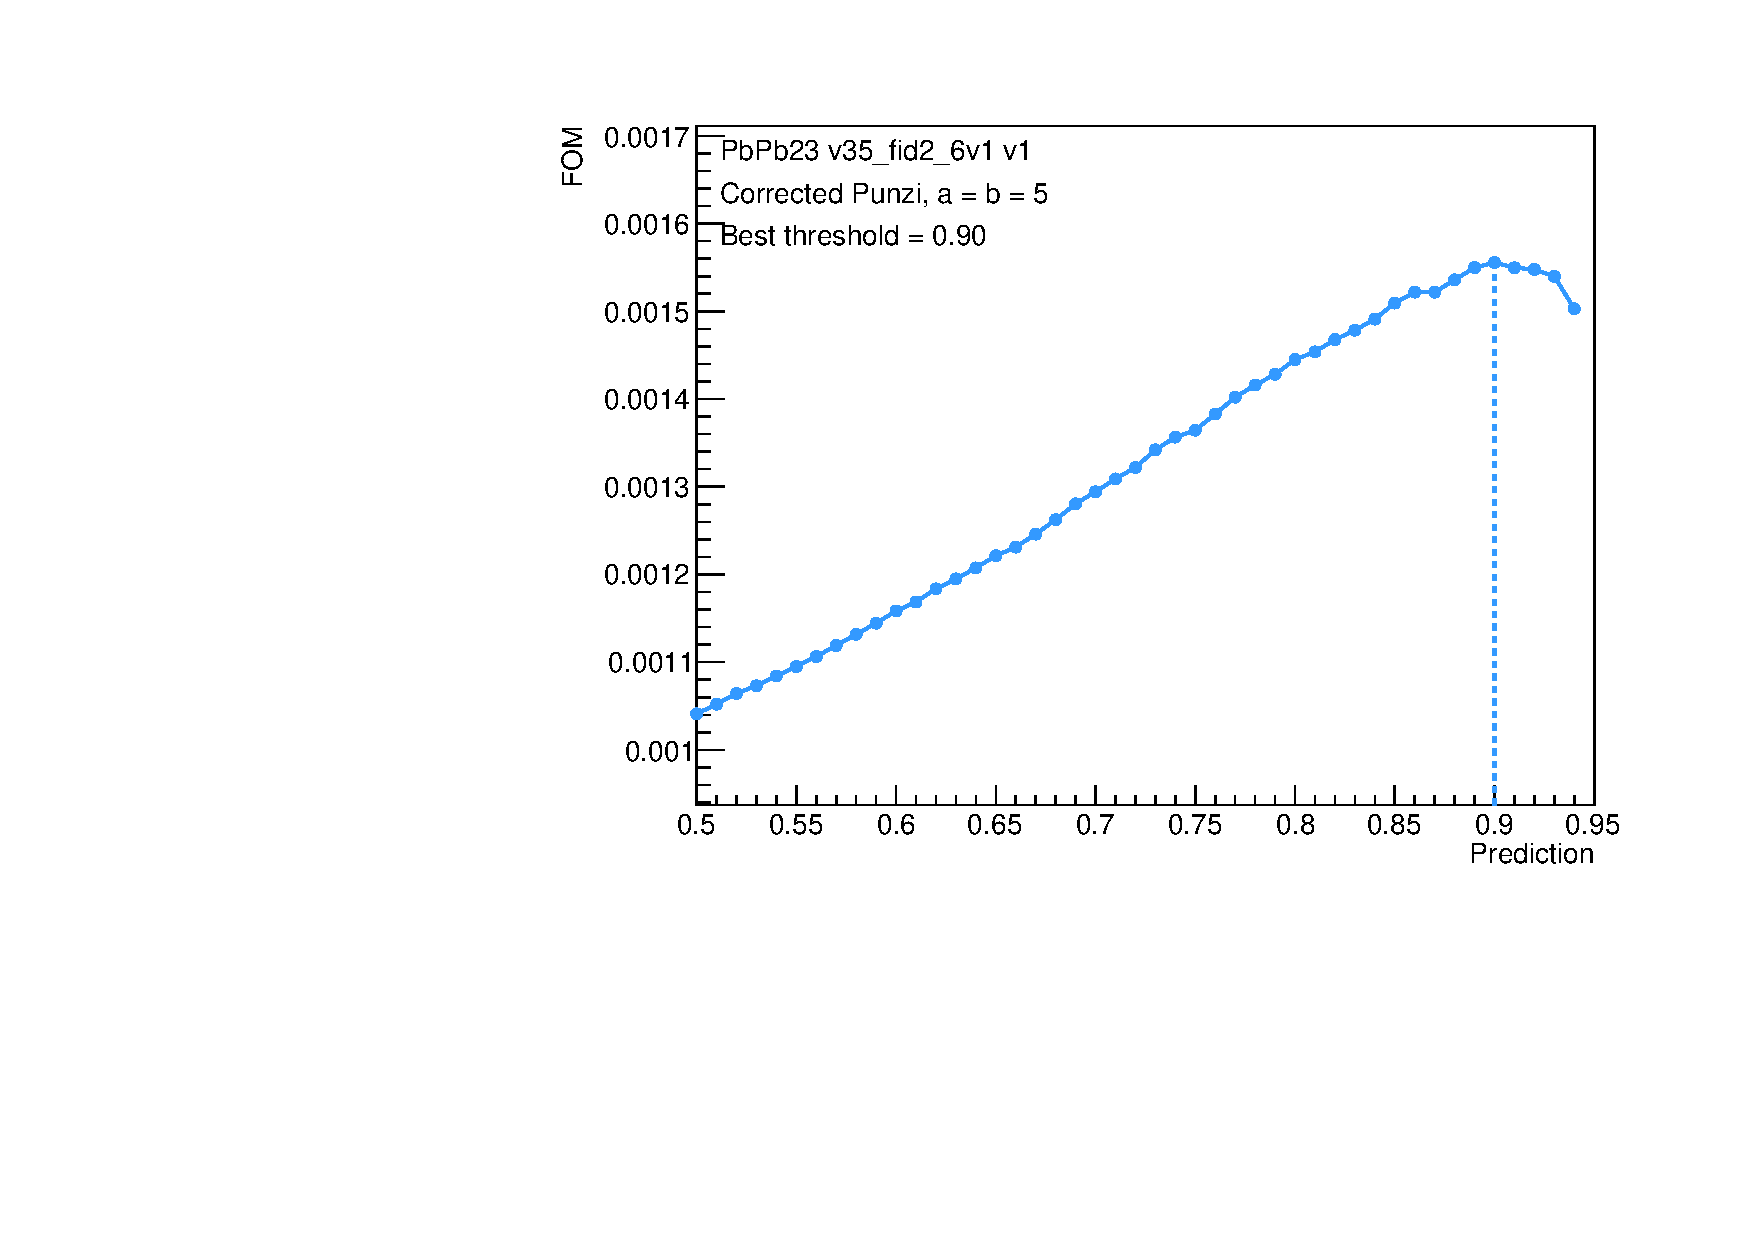
\includegraphics[width=\linewidth,height=0.73\textheight,keepaspectratio]{figures/20260924/backup_6v1_punzi_score.pdf}
\column{0.29\textwidth}\small
\textbf{Empirical corrected Punzi}\par
$a=b=5$.\par\medskip
Score: 0.50--0.95\par
Step: 0.01\par\medskip
\textbf{Grid maximum}\par
score $>0.90$\par
FOM $=1.555545\times10^{-3}$\par\medskip
\end{columns}
\end{frame}

\begin{frame}[label=u2_fit_2]{Six variables, pthat5 excluded: optimal two-peak fit}
\begin{columns}[T]
\column{0.65\textwidth}\centering
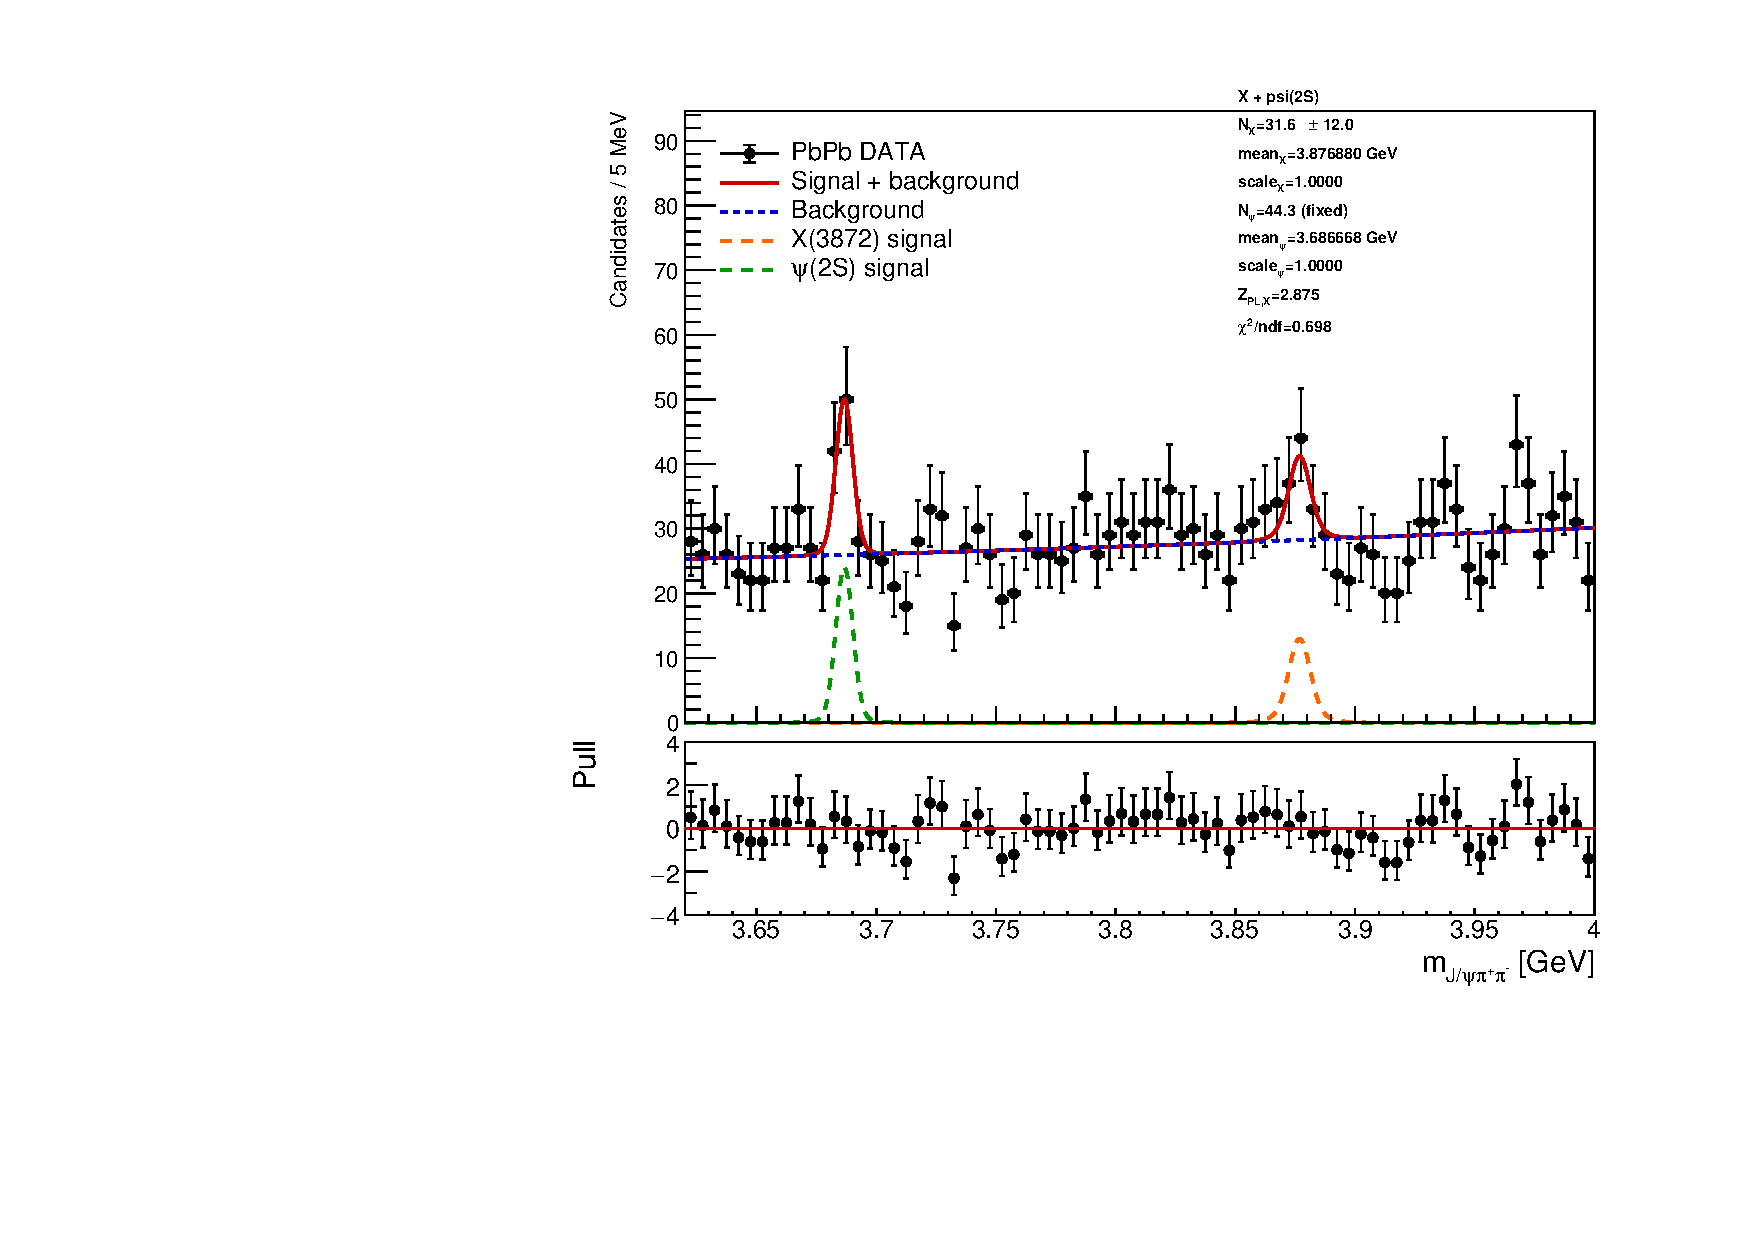
\includegraphics[width=\linewidth,height=0.72\textheight,keepaspectratio]{figures/20260924/backup_6v1_conditional_fit.pdf}
\column{0.32\textwidth}\small
\textbf{score $>0.90$}\par\medskip
$N_X=31.62\pm11.97$\par
$N_{\psi(2S)}=44.33$ (fixed)\par\medskip
$\sqrt{q_0}=2.875$\par
\medskip
MC double-Gaussian widths fixed.\par
2nd-order Chebyshev background.
\end{columns}
\end{frame}

\begin{frame}[label=u2_selection_3]{Five variables, pthat5 excluded: training}
\begin{columns}[T]
\column{0.46\textwidth}\small
\textbf{Common training selection}
\begin{center}
\begin{tabular}{@{}ll@{}}\toprule
Variable & Selection before ML\\\midrule
\var{Bpt} & $15 < \var{Bpt} < 50$ GeV\\
\var{By} & $|\var{By}| < 1.6$\\
\var{BQvalue} & $\var{BQvalue} < 0.15$ GeV\\
\var{Btrk2dR} & $\var{Btrk2dR} < 0.35$\\\bottomrule
\end{tabular}\end{center}
\column{0.50\textwidth}\small
\textbf{Input variables}\par\medskip
\var{Bmu1pt}, \var{Bmu2pt}\par
\var{Btrk2Pt}, \var{BtrkPtimb}\par
\var{Btrk1dR}\par\medskip
\textbf{X MC:} pthat5 excluded in training and application.\par
\var{pThatreweight}; no extra reweighting.\par
No additional signal training mass window.\par\medskip
\textbf{DATA training background}\par
$(3.80,3.85)\cup(3.89,3.94)$ GeV.\par
Unit weights; same common selection.
\end{columns}
\end{frame}

\begin{frame}[label=u2_punzi_3]{Five variables, pthat5 excluded: Punzi FOM}
\begin{columns}[T]
\column{0.68\textwidth}\centering
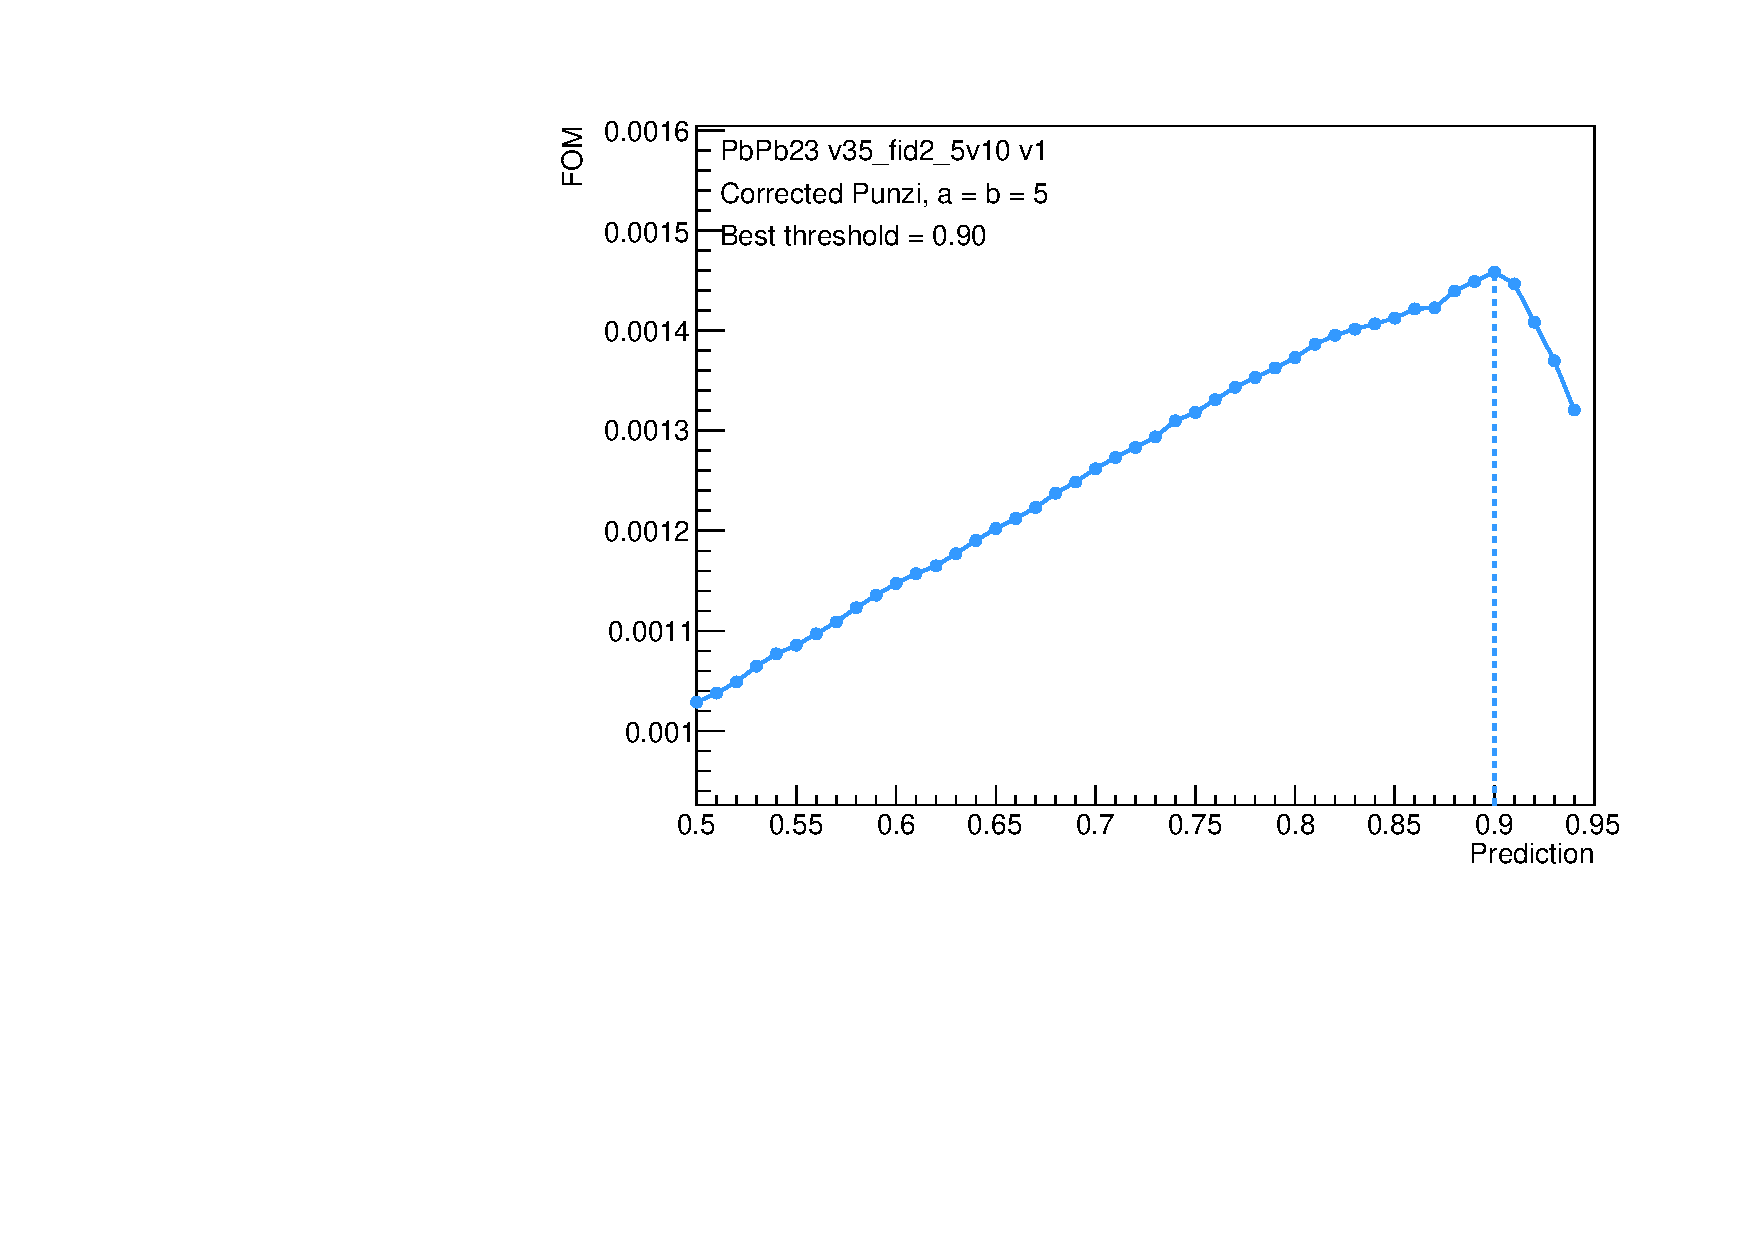
\includegraphics[width=\linewidth,height=0.73\textheight,keepaspectratio]{figures/20260924/backup_5v10_punzi_score.pdf}
\column{0.29\textwidth}\small
\textbf{Empirical corrected Punzi}\par
$a=b=5$.\par\medskip
Score: 0.50--0.95\par
Step: 0.01\par\medskip
\textbf{Grid maximum}\par
score $>0.90$\par
FOM $=1.458448\times10^{-3}$\par\medskip
\end{columns}
\end{frame}

\begin{frame}[label=u2_fit_3]{Five variables, pthat5 excluded: optimal two-peak fit}
\begin{columns}[T]
\column{0.65\textwidth}\centering
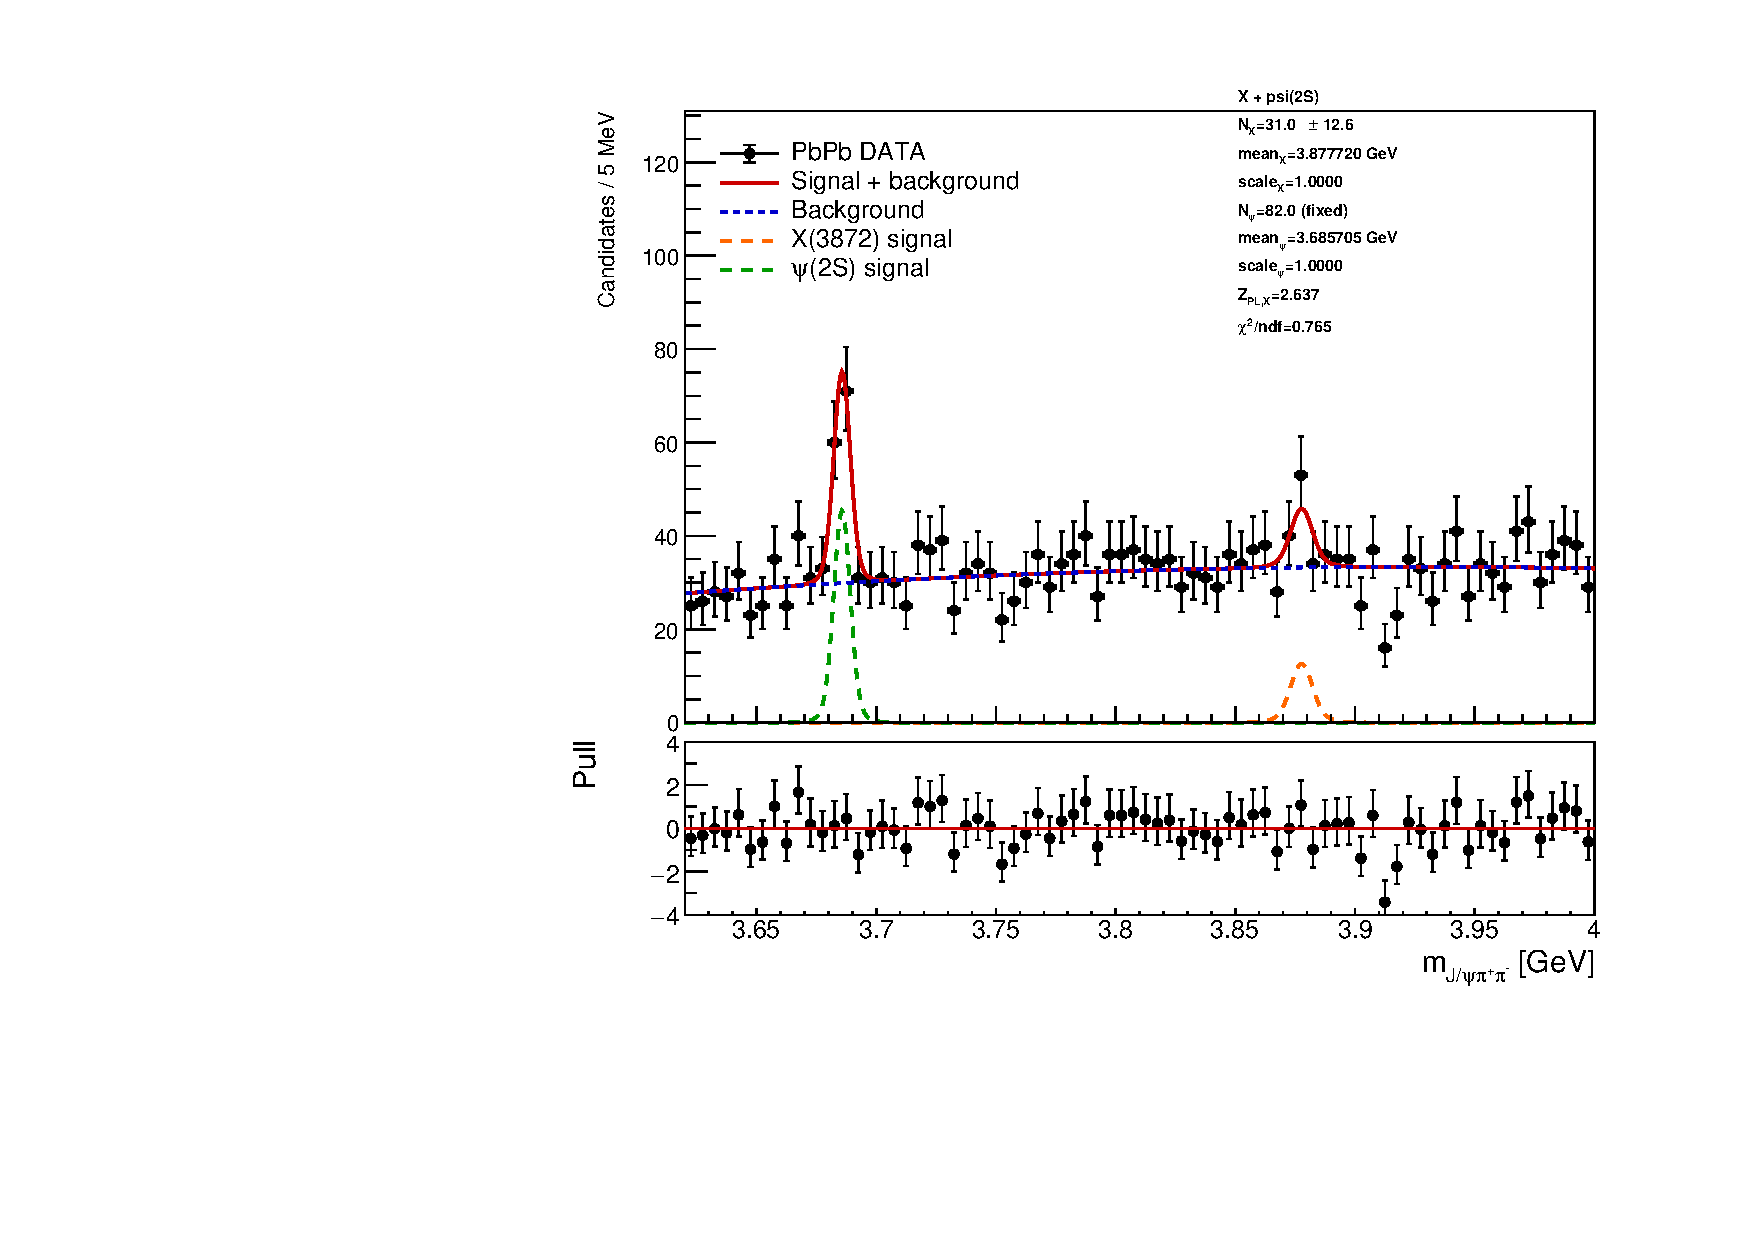
\includegraphics[width=\linewidth,height=0.72\textheight,keepaspectratio]{figures/20260924/backup_5v10_conditional_fit.pdf}
\column{0.32\textwidth}\small
\textbf{score $>0.90$}\par\medskip
$N_X=30.96\pm12.62$\par
$N_{\psi(2S)}=82.02$ (fixed)\par\medskip
$\sqrt{q_0}=2.637$\par
\medskip
MC double-Gaussian widths fixed.\par
2nd-order Chebyshev background.
\end{columns}
\end{frame}

